\chapter{Numerical experiments}
\label{chap:expe}

From the point of view of computational cost, it is convenient to make a brief analysis of the relevant new continuous-time framework obtained in \eqref{eqn:u3.3}. The main problem when dealing with large networks (matrices) resides in the computation of the matrix logarithm, which can be computationally expensive.

The matrix logarithm can be approximated by its Taylor series expansion. The Taylor series expansion of the matrix logarithm of $\mathbf{I} - \alpha \mathbf{A}$ can be expressed as:

$$\log(\mathbf{I} - \alpha \mathbf{A}) = \sum_{k=1}^{\infty} (-1)^{k+1}\frac{\alpha^k}{k}\mathbf{A}^k$$

where $\mathbf{I}$ is the identity matrix of size $N$. The accuracy of the approximation depends on the value of $k$, which determines how many terms in the series are included. The higher the value of $k$, the more accurate the approximation, but also the more computationally expensive it is to compute.

It is worth noting that for certain matrices, the Taylor series expansion may not converge or may converge too slowly to be practical for approximating the matrix logarithm. In such cases, other approximation methods like the Padé approximation or Schur decomposition may be more effective \cite[Ch.\ 11]{higham2008functions}.

In Python, the \texttt{scipy.linalg.logm} module from the SciPy library computes the logarithm of a matrix using a inverse scaling and squaring method together with a Schur decomposition with a computational cost of $\mathcal{O}(N^3)$ for an $N \times N$ matrix. However, the Schur decomposition is not always the most efficient way to compute the matrix logarithm, especially for large matrices with special properties such as sparsity or symmetry. In these cases, specialized algorithms, based on Krylov methods, rational approximations or iterative methods with preconditioning, may be used to approximate the matrix logarithm to reduce its computational cost. 

In this section, we consider first the two synthetic experiments from \cite{grindrod2014dynamical} in order to demonstrate how our new matrix ODE approach works and provide a better understanding of the $\alpha,\beta$ parameters. The \textit{synthetic} concept in these two experiments refers to the fact that they are based on artificially created networks with a simple and well-known structure of nodes. By comparing expected results with the actual ones obtained in the experiments, we will be able to test, validate and refine the new dynamic framework. The relatively small size of these examples, $N=31$ and $N=17$ nodes respectively, will facilitate the process of visualizing, and it will also allow us to employ a highly precise Runge-Kutta iteration to solve the corresponding ODE systems (\ref{eqn:u3.3}) with accuracy.

The new model is also examined in a third experiment based on real voice call data from the IEEE VAST 2008 Challenge \cite{grinstein2008vast}. Here, we try to find out if the new dynamic measures of centrality are able to identify hubs of influence in a large communication network ($N=400$), and if they offer a better perspective of the network evolution than static or aggregate measures.

For the initial two experiments, where there are only a few nodes, the Schur decomposition-based \texttt{scipy.linalg.logm} Python function is used to compute the matrix logarithm. However, when dealing with a larger number of nodes, as in the voice call experiment, a Taylor series approximation is considered to be a more effective approach to enhance computational efficiency.

\section{First synthetic experiment}
\label{sec:synexp1}

The first synthetic experiment models a cascade of information through the directed binary tree structure with $N=31$ nodes illustrated in Fig. \ref{fig:exp1}. On a time interval $t \in [0,20]$, the adjacency matrix $\mathbf{A}(t)$ of such network switches ten times between two constant values $\mathbf{A}_{even}$ and $\mathbf{A}_{odd}$ on each sub-interval $[i, i + 1)$ for $i=0,1,2,\dots$, specifically

\begin{equation*}
\mathbf{A}(t)\coloneqq
    \begin{cases}
        \mathbf{A}_{even}, & \text{if } \mod(\lfloor t \rfloor, 2) = 0\\
        \mathbf{A}_{odd}, & \text{otherwise} 
    \end{cases}
\end{equation*}

where $\lfloor t \rfloor$ denotes the floor function, $\mathbf{A}_{even}$ the adjacency matrix relative to the subgraph with solid edges in Fig. \ref{fig:exp1}, and $\mathbf{A}_{odd}$ the one relative to the subgraph with dashed edges. During the time an edge from node $i$ to node $j$ is active the respective entry of the adjacency matrix is set to $\mathbf{A}(t)_{ij}=1$, and zero otherwise. As we are dealing with directed links, $\mathbf{A}(t)_{ij}\ne \mathbf{A}(t)_{ji}$. This results in asymmetric matrices $\mathbf{A}(t)\in \mathbb{R}^{31\times 31}$ where most of their elements are zero and only a few entries belonging to the active nodes are set to one. More specifically, the non-zero entries of each adjacency matrix are given by $\mathbf{A}_{i,2i} = \mathbf{A}_{i,2i+1} = 1$ for $i \in \mathbb{S}(t)$, where 

\[
\mathbb{S}(t) =
    \begin{cases}
        \{ 1,4,5,6,7 \} & \text{if } \mod(\lfloor t \rfloor, 2) = 0, \\
        \{ 2,3,8,9,10,11,12,13,14,15 \} & \text{otherwise} 
    \end{cases}
\]

Some noise is added to this structure by including extra directed edges that are chosen uniformly at random for each subinterval, with an average of five edges added each time (see Appendix \ref{chap:appa} - Python code, l.28).

\begin{figure}[h]\centering
    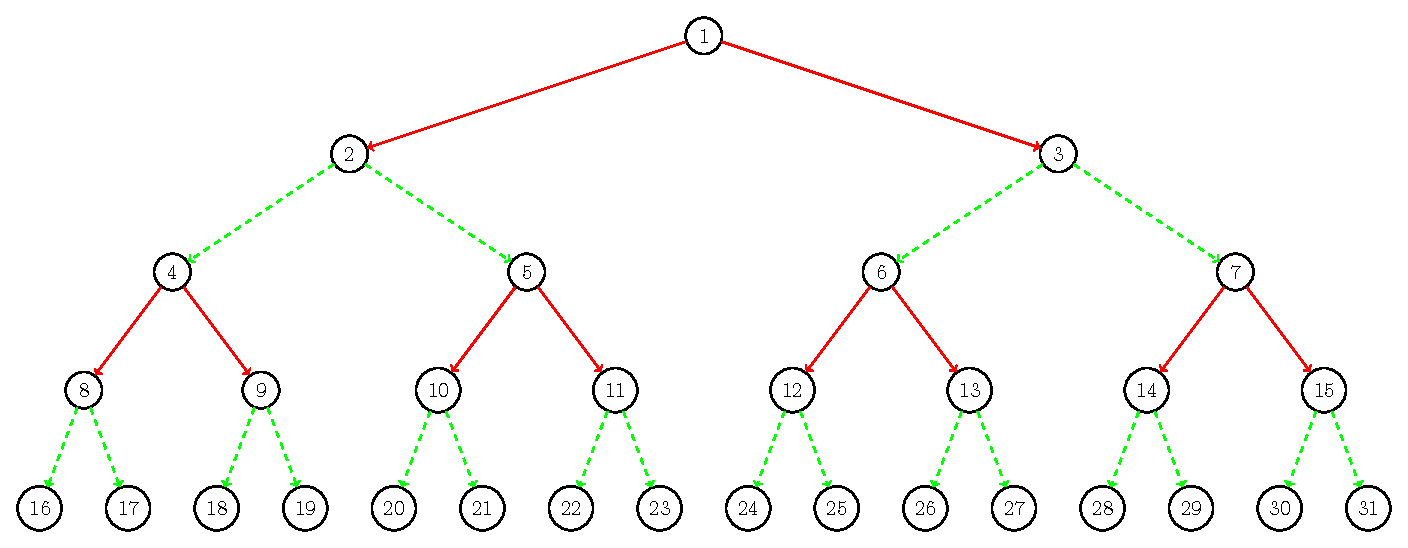
\includegraphics[width=.75\textwidth]{experiment1}
    \caption{Network structure (binary tree) for the first synthetic experiment. The active links of $\mathbf{A}(t)$ alternate between the solid and dashed edges, with extra noise added at each time step, over a period of 10 cycles.}
    \label{fig:exp1}
    \bigskip
\end{figure}

With this experiment, two main objectives are sought. First, to have a better understanding of what role $\alpha$ and $\beta$ parameters play. And second, to confirm that our model captures the cascade effect in the network along a hierarchy of influence that is hidden from a static or aggregate view.

For that purpose, four experiments were run to compute the dynamic broadcast centrality at $t=20$ for each node through \eqref{eqn:u3.3}--\eqref{eqn:u3.4}, varying only the values of $\alpha$ and $\beta$ as shown in Table \ref{table:parameters}. Note that the last experimental run does not consider any parameter as it is based on the computation of aggregate measures, in this case, the aggregate out degree represented by row sums of the aggregate adjacency matrix for the whole interval $t\in[0,20]$. By analyzing the eigenvalues of all generated $\mathbf{A}_{even}$ and $\mathbf{A}_{odd}$ it is seen that the maximum of the spectral radii of these matrices is 1, and therefore the solution to \eqref{eqn:u3.3} is well defined for $\alpha\in(0,1)$. The SciPy’s \texttt{solve\_ivp} method was used to numerically solve the matrix ODE, which uses an explicit Runge-Kutta method of order 5(4). Relative and absolute tolerances were left to their default values, $atol= 10^{-6}$ and $rtol=10^{-3}$. 

\begin{table}[ht]
            \bigskip
		\centering % used for centering table
		\begin{tabular}{c c c c c} % centered columns (4 columns)
			\hline\hline %inserts double horizontal lines
			\textbf{Parameter} & \textbf{\#1} & \textbf{\#2} & \textbf{\#3} & \textbf{\#4} \\ [0.1ex] % inserts table
			%heading
			\hline\hline 
			$\mathbf{\alpha}$ & 0.7 & 0.7 & 0.1 & -\\ % inserting body of the table
			$\mathbf{\beta}$ & 0.1 & 0.01 & 0.1 & - \\ [0.5ex] % [1ex] adds vertical space
			\hline %inserts single line
		\end{tabular}
		\caption{First synthetic experiment: Choice of the $\alpha,\beta$ parameters for the different experimental runs.} 
       \label{table:parameters} 
\end{table}

\newpage

Fig. \ref{fig:bt1} displays the dynamic broadcast centrality from \eqref{eqn:u3.4}, at time $t=20$ for each of the 31 nodes for  $\alpha=0.7$ and $\beta=0.1$. We observe that node 1 has a strong advantage in terms of centrality, and that centrality tends to decrease as the index increases. Nodes 2 and 5 are ranked higher than node 3, indicating that the additional noise has affected this part of the network.

Fig. \ref{fig:bt2} depicts the same results with a lower $\beta=0.01$ value, which increases the contribution of older walks. As a reminder, if we consider a walk starting at time zero, then the  downweighting factor becomes $e^{−20 \times 0.01} \approx 0.8$ rather than $e^{−20 \times 0.1} \approx 0.1$. This change of the $\beta$ parameter has a negligible effect on the node rankings which makes sense considering that the network dynamics have an underlying periodic pattern, but it can be observed that it generates larger absolute values.

In Fig. \ref{fig:bt3}, we return to the original $\beta=0.1$ value and set $\alpha=0.1$, resulting in less marked differences in the node rankings. Even though node 1 continues to be the most central, the differences are less pronounced as its capability to initiate numerous dynamic walks of length 4 to nodes at the bottom of the hierarchy has less influence or weight.

Fig. \ref{fig:bt4} illustrates the aggregate out degree of each node, that is, the sum of out degrees over time for each node. For nodes 1 to 15 in the binary tree structure, this value is 20 (2 active edges $\times$ 10 cycles), which fluctuates due to the introduced noise. 

Overall, this experiment allows us to clearly visualize the dynamic effect arising from the time-ordering of the node interactions. Due to the hierarchy and timing of the edges, information appears to flow from lower indices to higher. The binary structure of the tree makes node 1 particularly efficient at transmitting information through the network, although this is not immediately apparent in a single snapshot. The last plot highlights that the overall bandwidth in terms of the aggregate out degree of a node can be a misleading network metric for determining node influence.

\begin{figure}[h]
     \centering
     \begin{subfigure}[b]{0.49\textwidth}
         \centering
         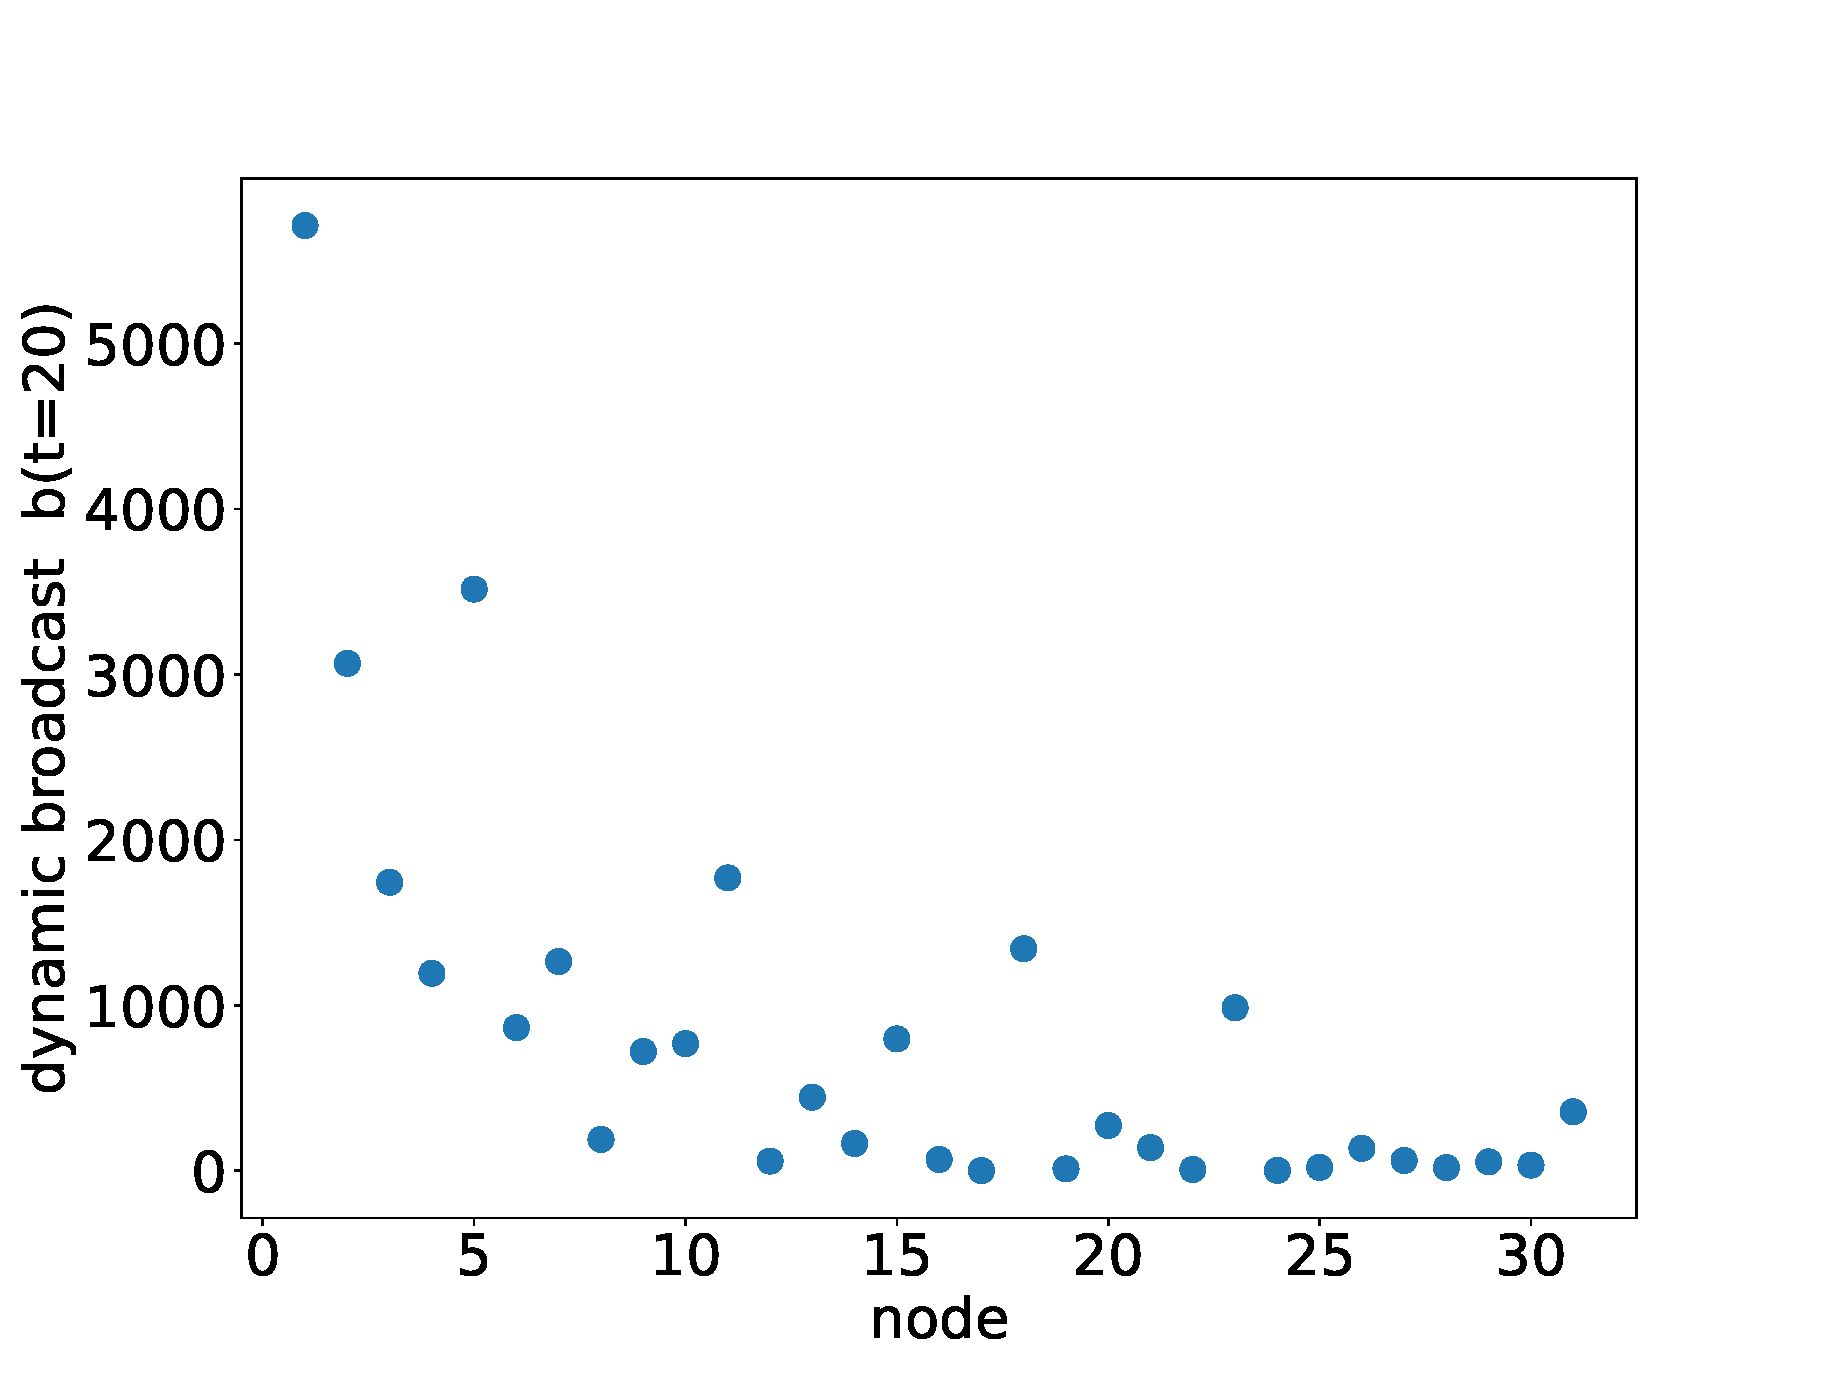
\includegraphics[width=\textwidth]{exp1_bt20a}
         \caption{Broadcast for each of the 31 nodes, $\alpha = 0.7 ,~\beta = 0.1$}
         \label{fig:bt1}
     \end{subfigure}
     %\hspace{0.1cm}
     \begin{subfigure}[b]{0.49\textwidth}
         \centering
         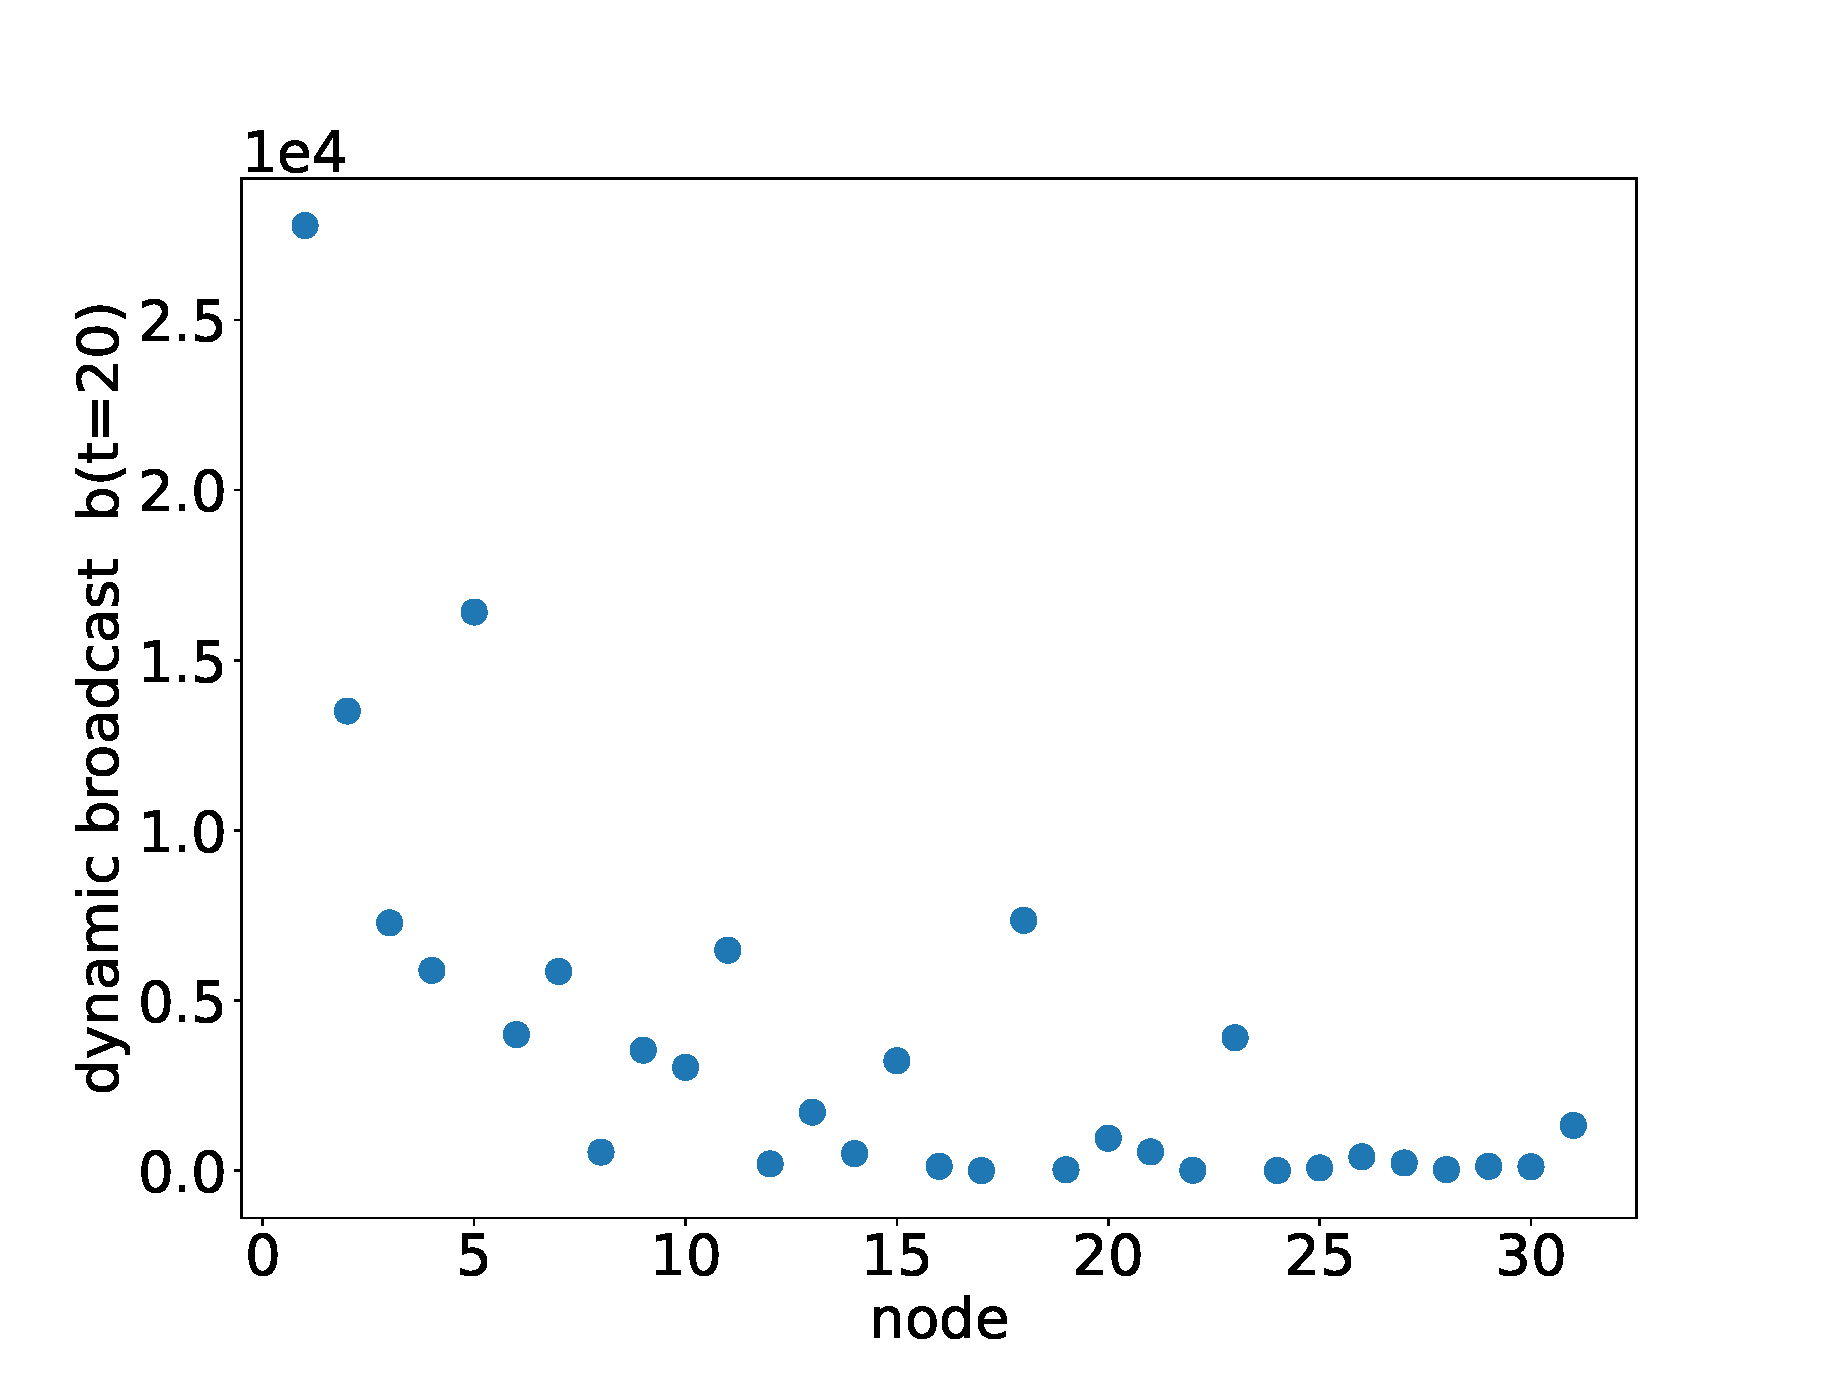
\includegraphics[width=\textwidth]{exp1_bt20b}
         \caption{Broadcast for each of the 31 nodes, $\alpha = 0.7 ,~\beta = 0.01$}
         \label{fig:bt2}
     \end{subfigure}
     
     \begin{subfigure}[b]{0.49\textwidth}
         \centering
         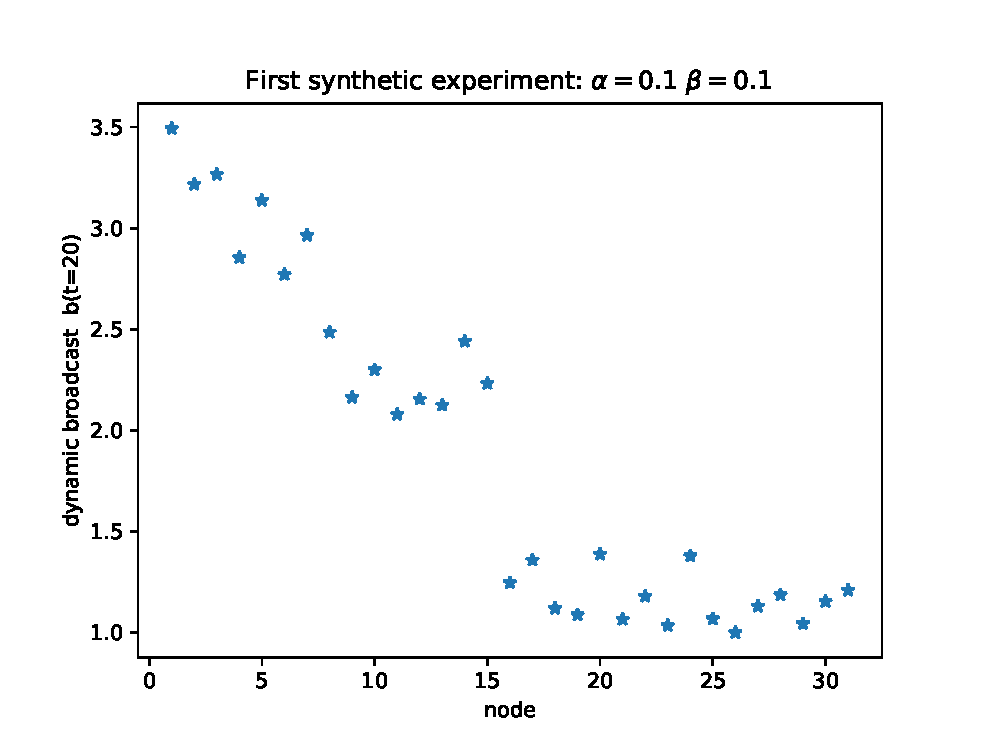
\includegraphics[width=\textwidth]{exp1_bt20c}
         \caption{Broadcast for each of the 31 nodes, $\alpha = 0.1 ,~\beta = 0.1$}
         \label{fig:bt3}
     \end{subfigure}
     %\hspace{0.1cm}
     \begin{subfigure}[b]{0.49\textwidth}
         \centering
         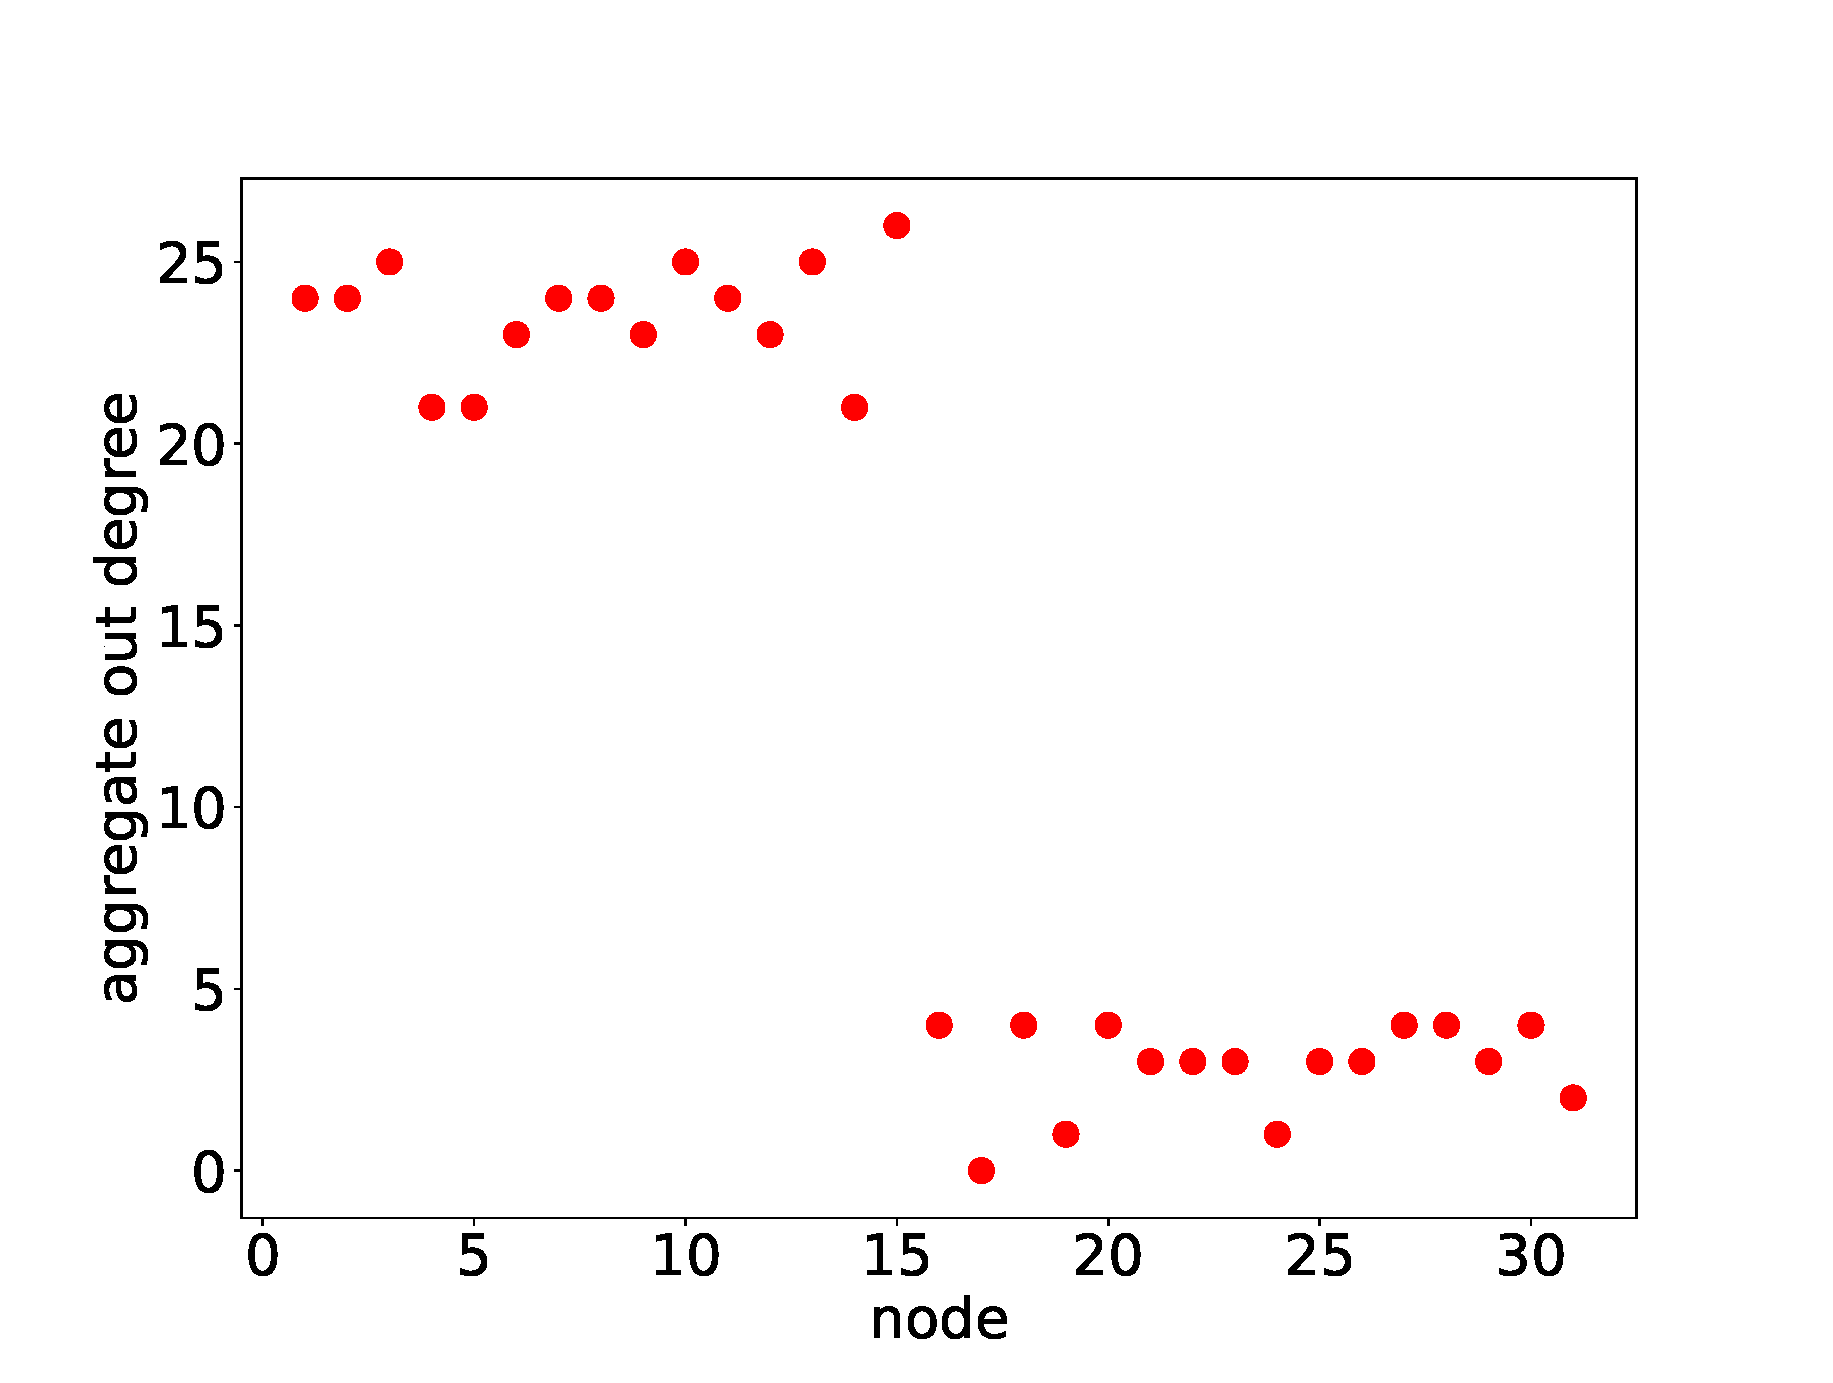
\includegraphics[width=\textwidth]{exp1_agg_out_degree}
         \caption{Aggregate out degree for each node}
         \label{fig:bt4}
     \end{subfigure}
        \caption{First synthetic experiment: results from the dynamic network in Fig. \ref{fig:exp1}.}
        \label{fig:fourbt}
\end{figure}

\section{Second synthetic experiment}
\label{sec:synexp2}
We now consider the second synthetic experiment from \cite{grindrod2014dynamical}. The experiment simulates multiple rounds of voice calls that occur along an undirected binary tree structure. Each node in the tree has at most one active edge at any given time, meaning that there are no "conference" calls. Fig. \ref{fig:exp2} shows the network of $N=17$ nodes with labels assigned to the edges indicating when they are active. The adjacency matrix, $\mathbf{A}(t)$, for this experiment is defined based on the ordered and non-overlapping time intervals such that $t_i\coloneqq[(i − 1)\tau , (i − 1 + 0.9)\tau )$, for $i=0, 1, \dots , 7$, and $\tau =0.1$.

\begin{figure}[h]\centering
    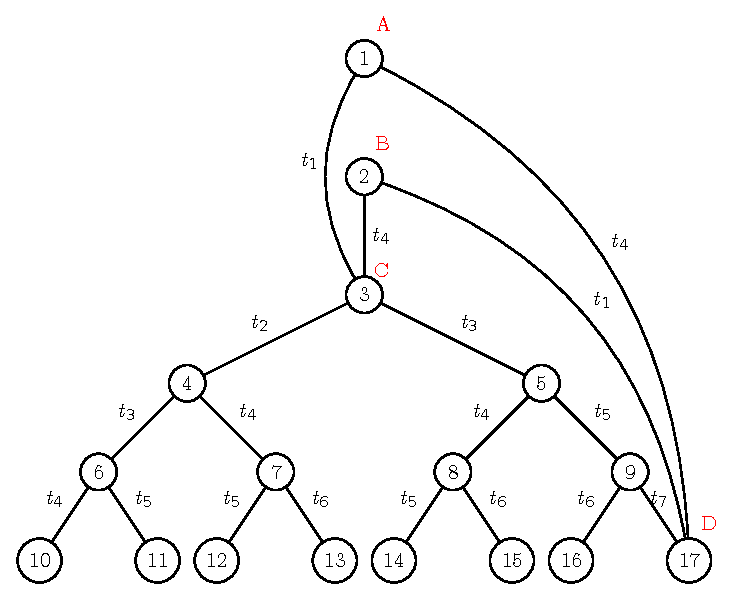
\includegraphics[width=.65\textwidth]{experiment2}
    \caption{Network structure for the second synthetic experiment. Links of $\mathbf{A}(t)$ are active over non-overlapping time intervals such that $t_i\coloneqq[(i − 1)\tau , (i − 1 + 0.9)\tau )$, for $i=0, 1, \dots , 7$, and $\tau =0.1$, repeated periodically over five cycles.}
    \label{fig:exp2}
    \bigskip
\end{figure}

The dynamic network is constructed in a way that node A (node 1) is designed to be a more effective influencer compared to node B (node 2). This can be attributed to several factors such as a higher social/business status or access to more current and relevant information. Connections are built in such a way that node A talks to node C (node 3) in $t_1$, initiating a cascade of phone calls in the network. On the other hand, node B communicates with node D (node 17) at $t_1$ and waits until $t_4$ to contact node C, which does not trigger any new cascades. The experiment is repeated over five cycles, during which nodes A and B send out a total of 10 messages. 

What we expect from this experiment, and makes it different from the previous one, is to verify that our continuous-time framework is capable of revealing the differences in terms of dynamic broadcast centrality between the node A that enjoys a cascade effect of information in the network and node B that does not. Even if these nodes have an apparent identical behaviour from an overall perspective, both contacting nodes C and D for the same length of time.

As pointed out in the remark on the role of the $\alpha$ and $\beta$ parameters, in the scenario of undirected one-to-one communication, such as voice calls with no teleconferences, all the symmetric adjacency matrices turn out to have unitary spectral radius for each time interval. A complete definition of these matrices can be seen in Appendix \ref{sec:fse} - Second synthetic experiment, l.22. Values of $\alpha=0.7$ and $\alpha=0.9$ were chosen to compare centrality results keeping fixed the value of $\beta=0.1$ which does not play an important role in this experiment due to the underlying periodic pattern in the network dynamics (similar results were obtained for different values of $\beta$). 

Implementing \eqref{eqn:u3.3}--\eqref{eqn:u3.4} in Python, $\mathbf{b}(t)$ was computed for the interval $t\in[0,3.5]$ for nodes A and B, using the \texttt{solve\_ivp} function with default parameters: $method="RK45"$, $atol=10^{-6}$ and $rtol=10^{-3}$.

The results in Fig. \ref{fig:twobt} (for $\alpha = 0.7, \beta = 0.1$ and $\alpha = 0.9 , \beta = 0.1$ respectively) show that the dynamic broadcast centrality measure is able to capture the cascade effect enjoyed by node A (solid line) with respect to node B (dashed line). This difference in broadcast centrality is much more pronounced for values of $\alpha$ close to one (see Fig. \ref{fig:bt6}), where longer walks are more strongly penalized. 

\begin{figure}
     \centering
     \begin{subfigure}[b]{0.49\textwidth}
         \centering
         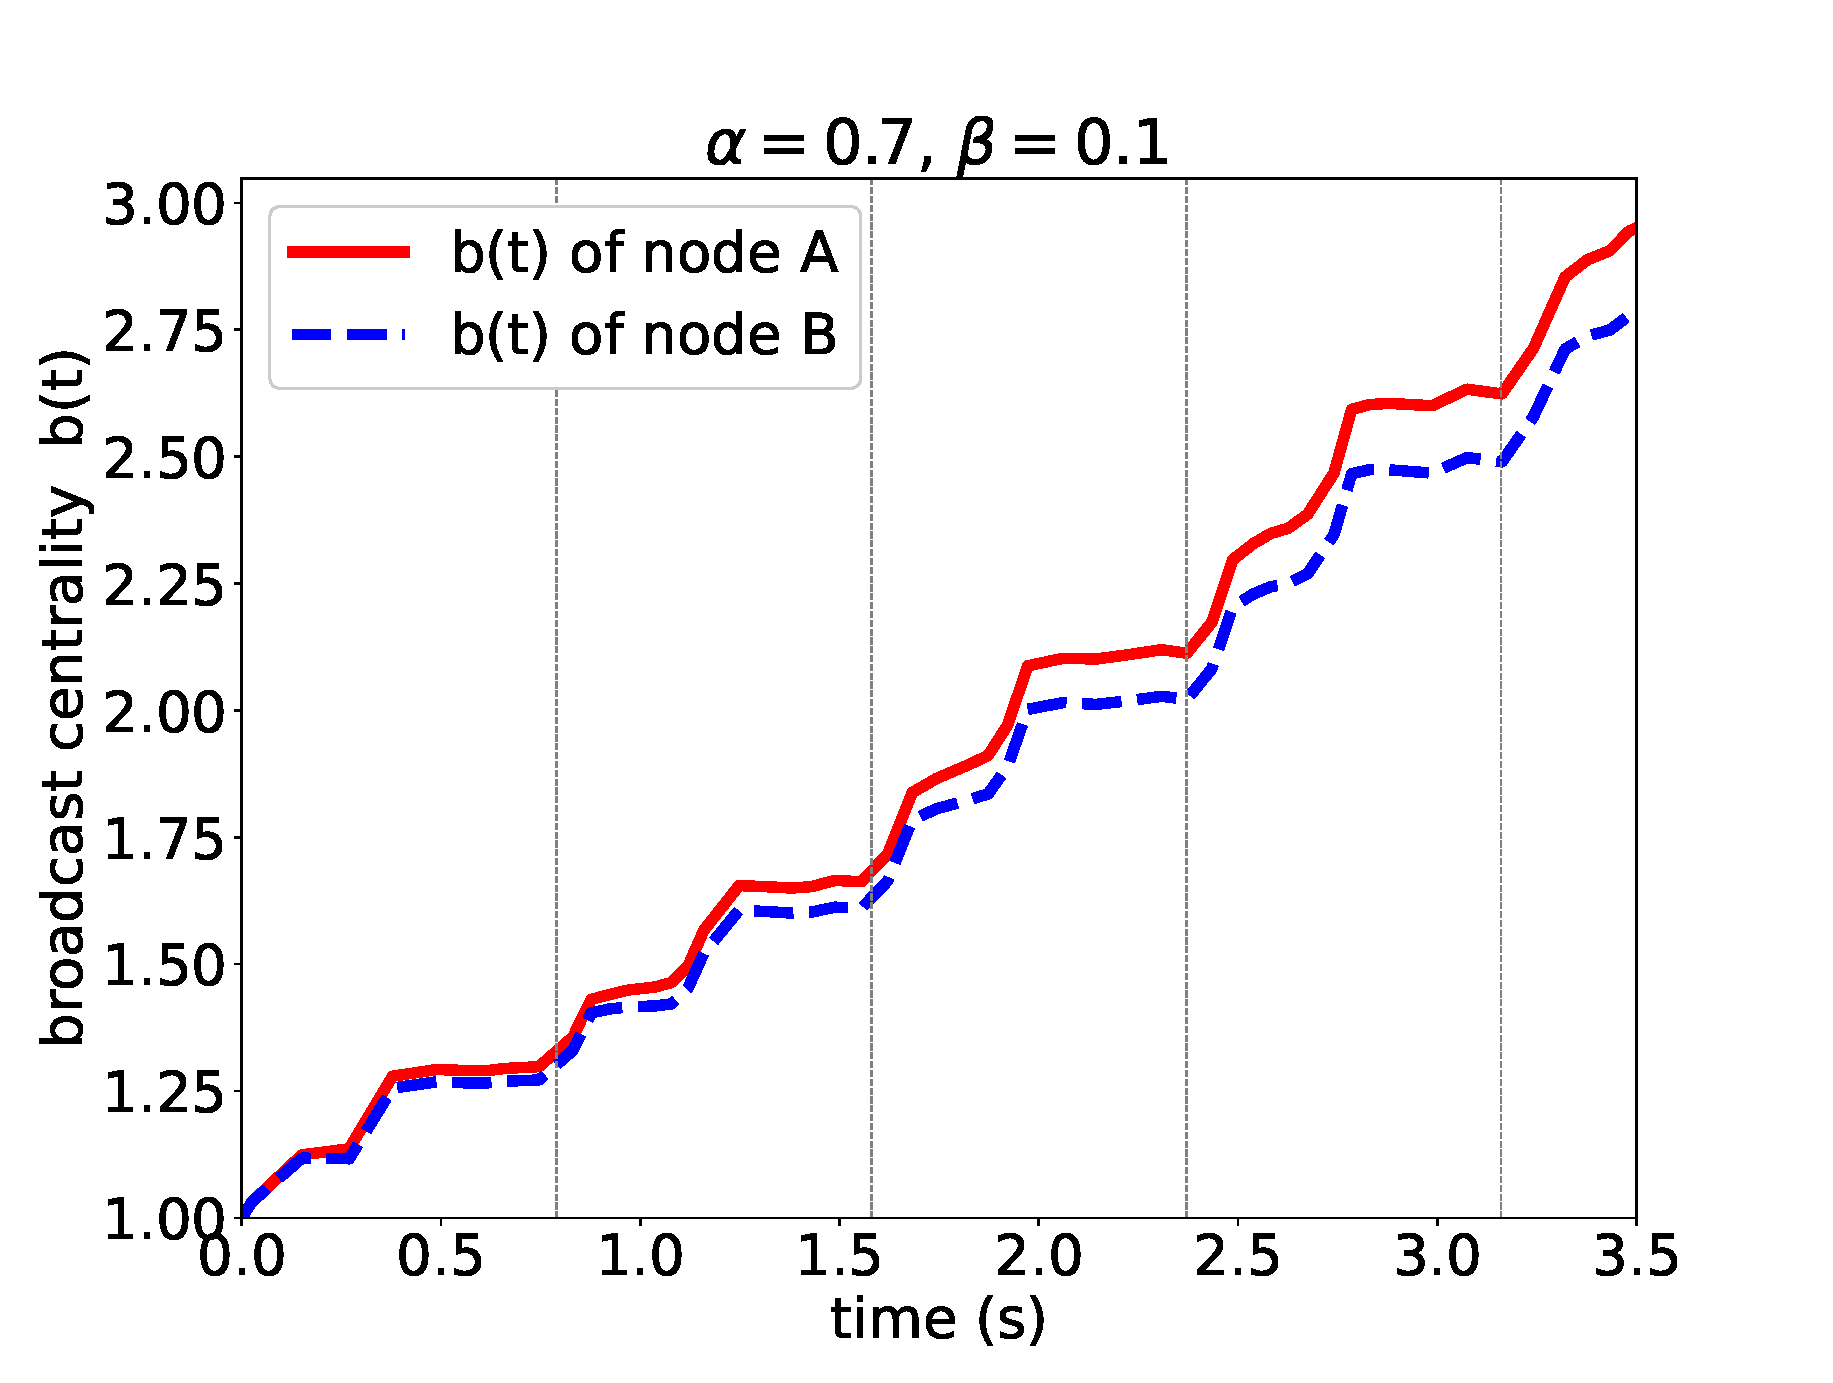
\includegraphics[width=\textwidth]{exp2b_btA_vs_btB}
         \caption{$\mathbf{b}(t)$ for $\alpha = 0.7 ,~\beta = 0.1$}
         \label{fig:bt5}
     \end{subfigure}
     \hfill
     \begin{subfigure}[b]{0.49\textwidth}
         \centering
         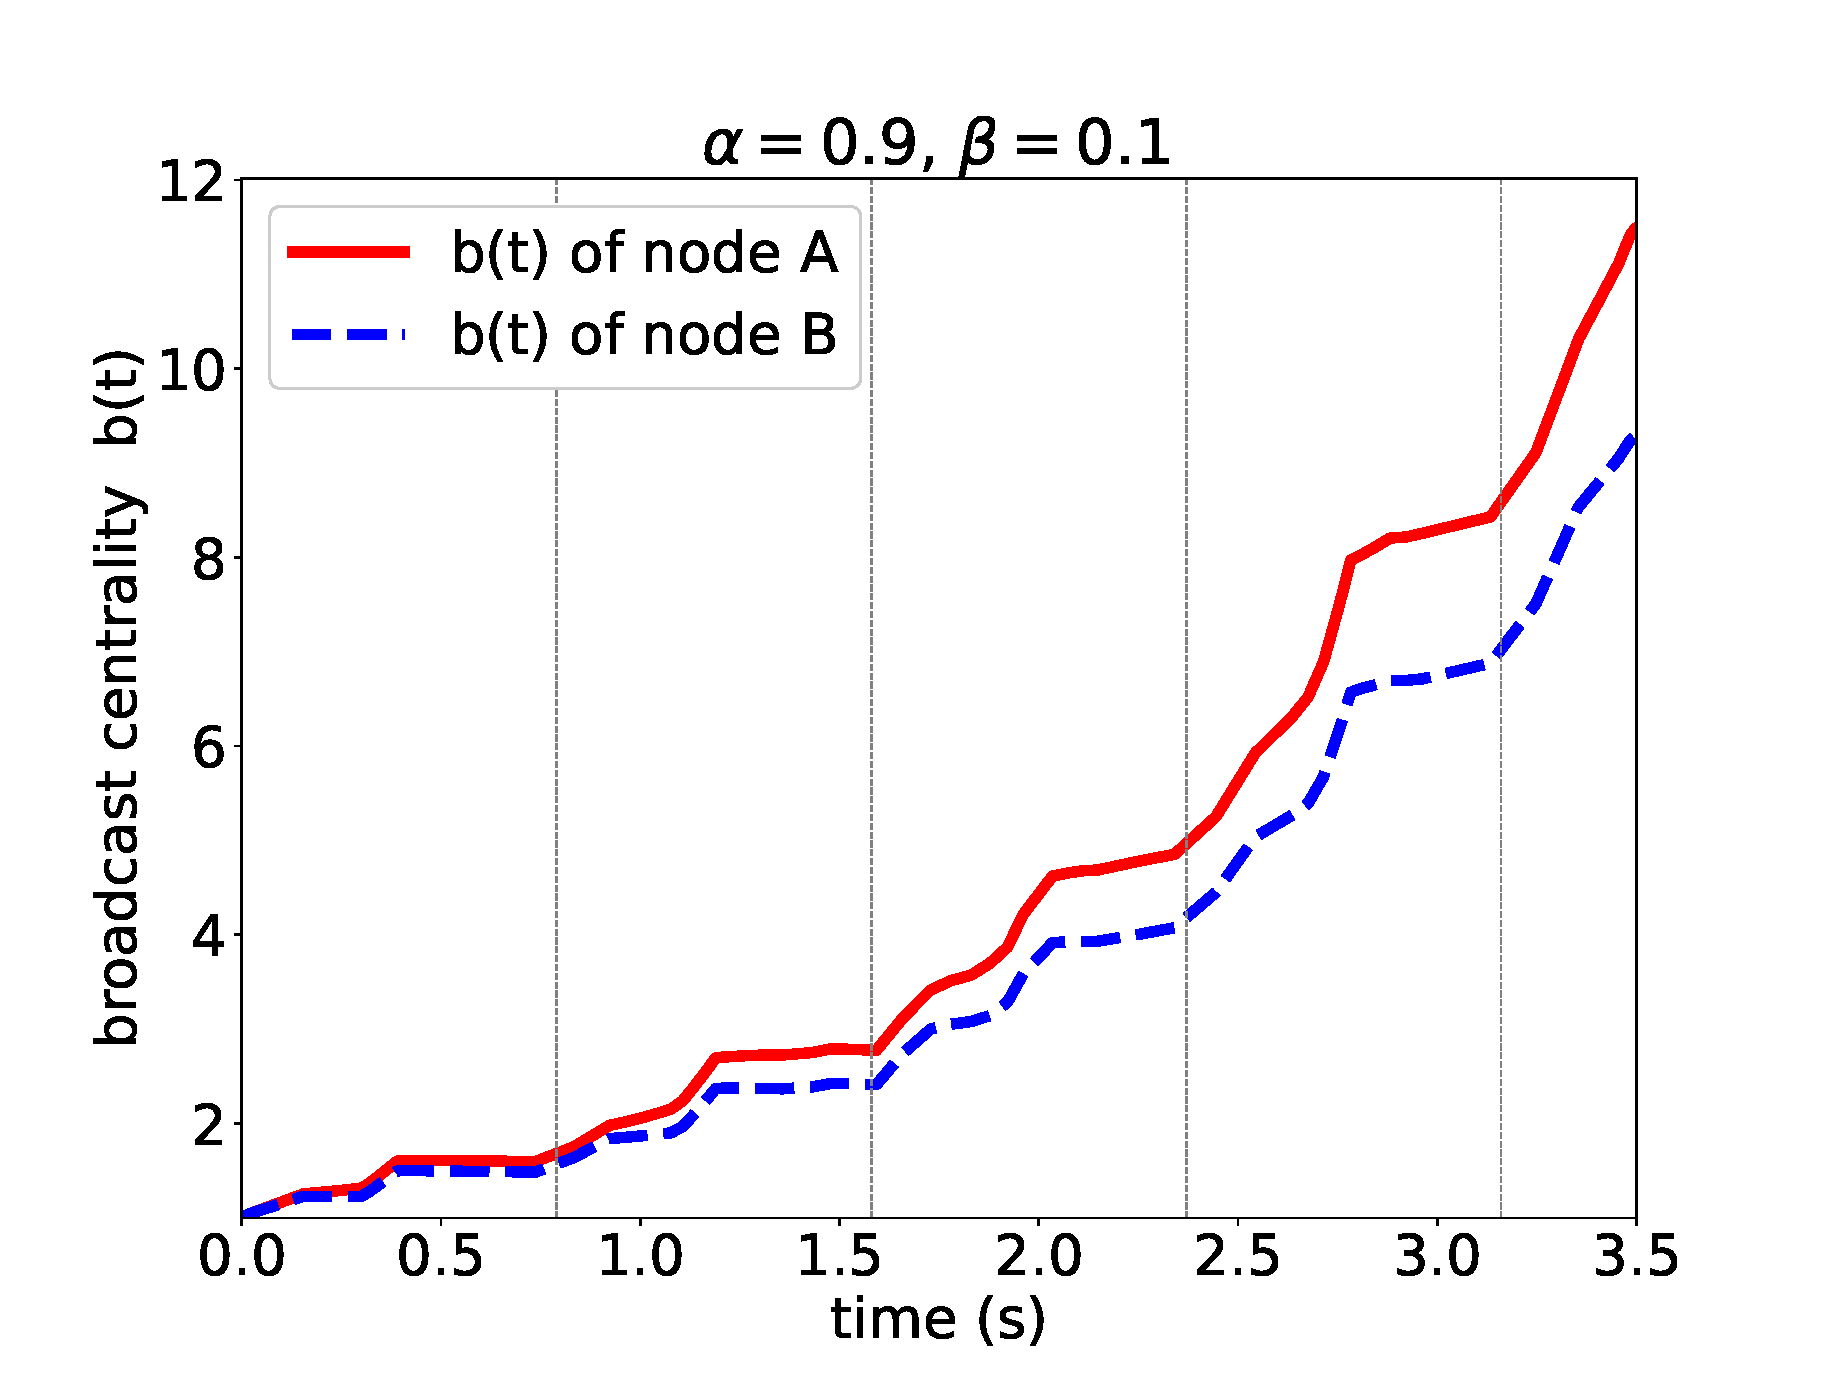
\includegraphics[width=\textwidth]{exp2a_btA_vs_btB}
         \caption{$\mathbf{b}(t)$ for $\alpha = 0.9 ,~\beta = 0.1$}
         \label{fig:bt6}
     \end{subfigure}
     \caption{Second synthetic experiment: dynamic broadcast centrality over time for node A (solid) and node B (dashed) in the network of Fig. \ref{fig:exp2}.}
     \label{fig:twobt}
\end{figure}

The iterative way in which the dynamic communicability matrix \eqref{eqn:dyncommatiter} is defined as a product of non-negative matrices based on the computation of the previous steps, ensures that nodes do not become less communicative over time. This characteristic is reflected in the increasing curves for both plots. This can also be interpreted from the fact that as time goes on, more nodes in the network will have received the message. Then, as more nodes receive the message, the number of nodes that can be reached in a single step will increase, and so will the broadcast centrality of the original node. Moreover, if we divide the plots into the five cycles that network communication is repeated by vertical lines, the particular staircase shape of the curves is explained by the fact that nodes A and B are active during $t_1$ and $t_4$ which causes a notable increase in broadcast centrality after these points.

As a curiosity, other nodes in this network, such as nodes 3, 4 and 5, offer greater centrality than nodes 1 (node A) and node 2 (node B). In fact, node 3 is the one with the highest centrality in the entire network. However, the main objective of this experiment was not to highlight this feature but to verify that our continuous-time ODE framework was capable of establishing a remarkable difference in the dynamic behavior between nodes A and B.

\section{Voice call experiment}
\label{sec:voicecall}
The next experiment applies the new modelling framework \eqref{eqn:u3.3} to a set of voice call interactions, in order to analyze the dynamic behavior of a fictitious, controversial socio-political movement. The data used for the experiment, supplied as part of the IEEE VAST 2008 Challenge \cite{grinstein2008vast}, consists of a complete set of 9834 time-stamped calls across 400 cell phone users over a 10 day period, with information on IDs for the send and receive nodes, start time in hours/minutes, and duration in seconds.

The aim of the experiment is to show the usefulness of the new matrix ODE in dealing with this type of dynamic network, comparing dynamical measures against aggregated. To that end, the bandwidth of a node is defined as the aggregate number of seconds for which the node ID is active as a sender or receiver. This will allow us to compare the effective activation time of a certain node with its relevance in terms of dynamic broadcast centrality.

The designers of the above mentioned competition provided additional information indicating that node 200 was the leader of an important community who controlled a closely connected subnetwork or inner circle consisting of nodes 1, 2, 3, and 5. However, starting from day 7, these individuals seem to have switched their phone IDs: node 200 became 300, and the others became 306, 309, 360, and 392.

For this experiment, $\mathbf{A}(t)$ was assumed to be symmetric, meaning that $\mathbf{A}(t)_{ij} = \mathbf{A}(t)_{ji} = 1$ if nodes $i$ and $j$ were communicating at time $t$, which was measured in seconds. Parameters $\beta$ was chosen to be approximately $\beta = 1/(60\times 60 \times 24) \approx 1.2 \times 10^{-5}$, which corresponded to a time downweighting of $e^{-1}$ per day, and set the edge attenuation parameter $\alpha$ to a similar value of $10^{-4}$. The SciPy's \texttt{solve\_ivp} method was again used to numerically solve the ODE (\ref{eqn:u3.3}) (see Appendix \ref{chap:appa} - Voice call experiment, l.257). Additionally, absolute and relative error tolerances were both set to $10^{-4}$. To improve efficiency, the matrix logarithm was approximated in this occasion with its expansion to the fifth power:

$$\log(\mathbf{I} - \alpha \mathbf{A}(t)) \approx \alpha \mathbf{A}(t) - \alpha^2 \mathbf{A}(t)^2/2 + \alpha^3 \mathbf{A}(t)^3/3 - \alpha^4 \mathbf{A}(t)^4/4 + \alpha^5 \mathbf{A}(t)^5/5$$ 

Visually speaking, the effects of increasing the number of terms in the expansion to 6 and 7 remained identical.

\begin{figure}[h]\centering
    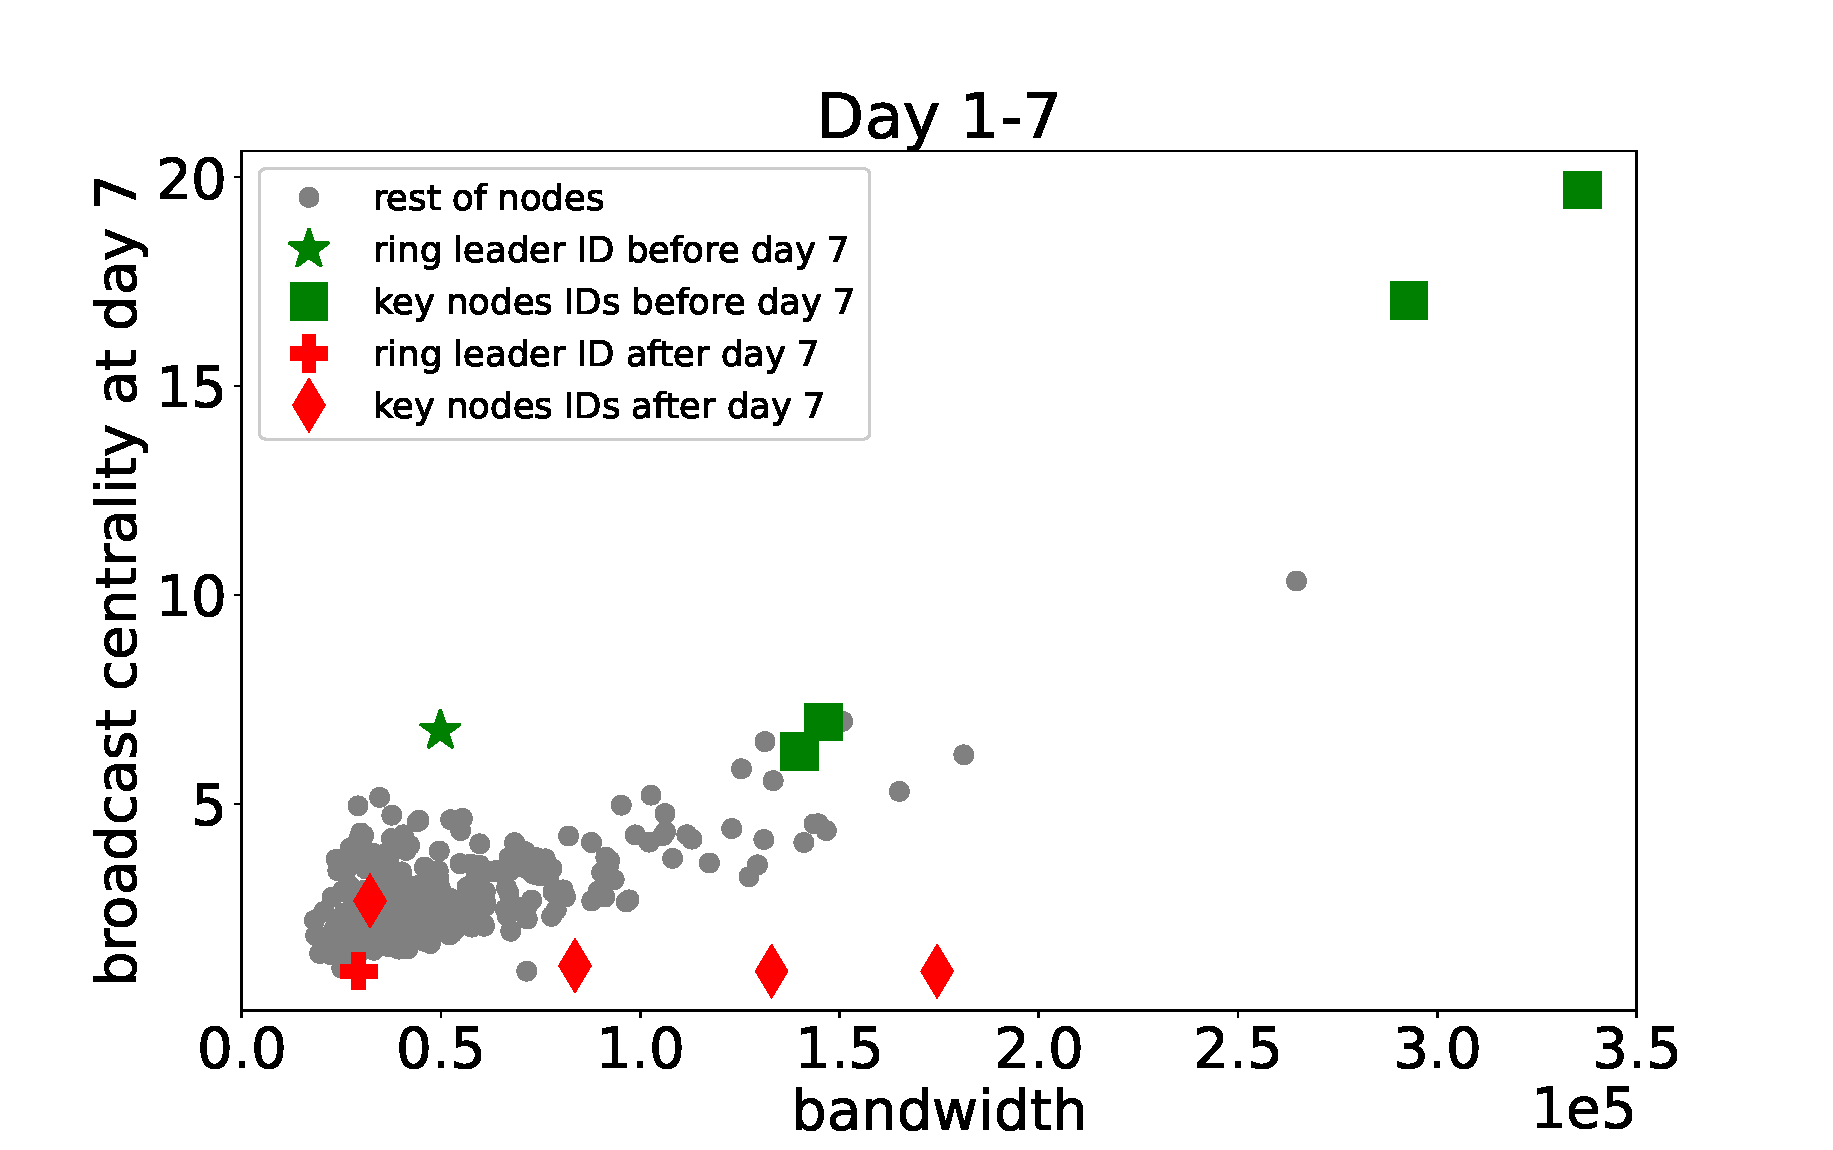
\includegraphics[width=.79\textwidth]{voicecall_exp_1_7}
    \caption{Voice call experiment: broadcast centrality for each node at the end of day 6 vs. bandwidth (secs.).}
    \label{fig:ve1a}
    \bigskip
\end{figure}

This experiment yields two key findings:
\begin{enumerate}[label=(\roman*)]
  \item The dynamic broadcast/receive measures \eqref{eqn:u3.4} are able to identify key nodes as highly influential, even if they are not actively using much bandwidth, without any prior knowledge of an inner circle's existence.
  \item The transformation that occurs in the network on day 7 is revealed by the running centrality measures once we know the IDs of the inner circle.
\end{enumerate}

Fig. \ref{fig:ve1a} was used to demonstrate point (i) by plotting bandwidth against dynamic broadcast, $\mathbf{b}(t)$, using data up until the end of day 6. The scatter plot also includes symbols to mark certain nodes, such as a star for the ring leader, 200, and squares for the related inner-circle nodes, 1, 2, 3, and 5. The follow-on ID for the ringleader, 300, is marked with a plus symbol, and those for other members, 306, 309, 360, and 392, are marked with diamonds.

The results showed that the key nodes for days 1-6 were much more dominant in terms of dynamic broadcast than overall bandwidth. Specifically, the ringleader node had a low bandwidth but ranked sixth out of 400 in terms of broadcast communicability.

\begin{figure}[h]\centering
    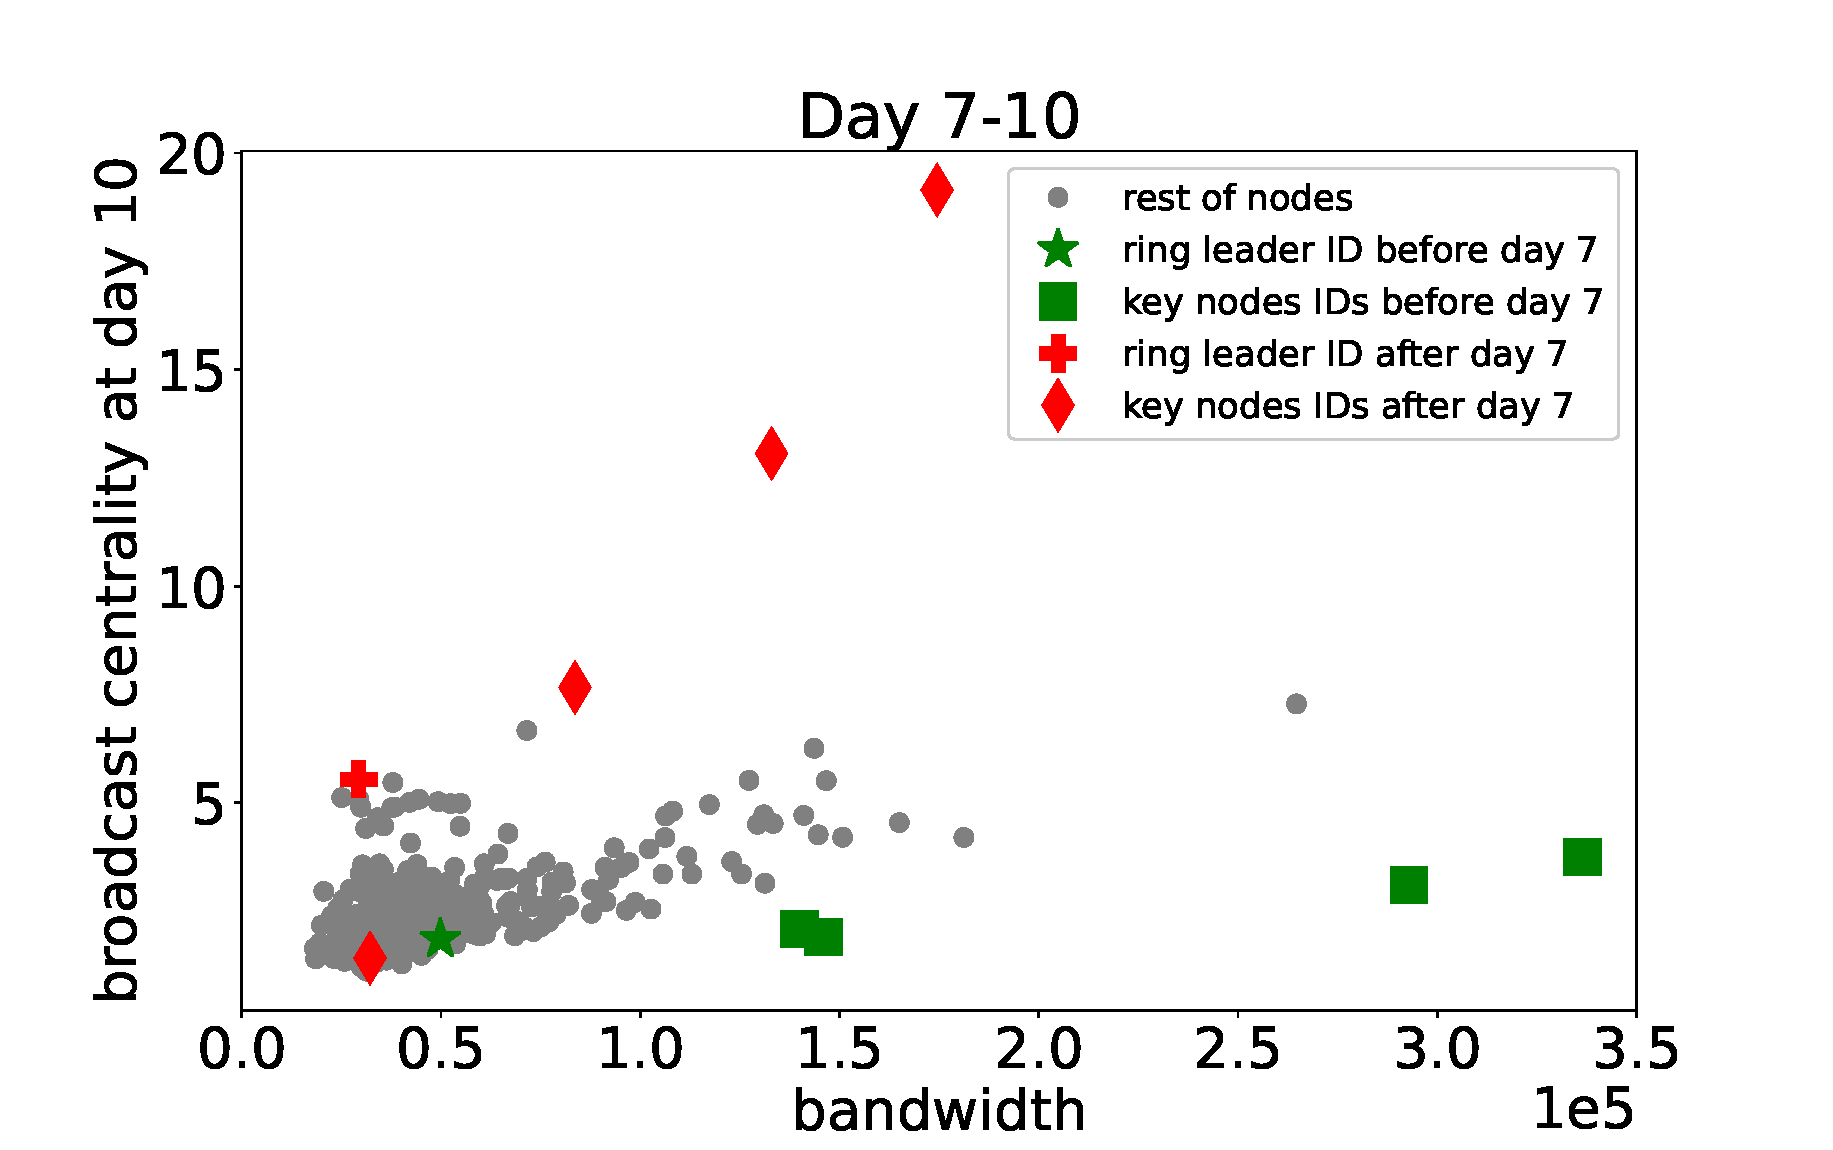
\includegraphics[width=.79\textwidth]{voicecall_exp_7_10}
    \caption{Voice call experiment: broadcast centrality for each node at the end of day 10 vs. bandwidth (secs.).}
    \label{fig:ve1b}
    \bigskip
\end{figure}

The data from days 7 to 10 is displayed in Fig. \ref{fig:ve1b}. The plot shows how the new ID of the ringleader, that is indicated by a plus symbol, has a low overall bandwidth, but ranks seventh highest for broadcast centrality. Although the former IDs from the inner circle, marked with diamonds, still possess high bandwidth, their low dynamic broadcast scores suggest that they are no longer central players. This experiment confirms that the dynamic broadcast score is a more effective indicator of centrality than overall bandwidth in uncovering the inner circle.

Dynamic receive centrality, $\mathbf{r}(t)$, was also computed using its own vector-valued ODE \eqref{eqn:u4.1} for data from days 1 to 7 obtaining similar results and a computation time reduction per function call of approximately $30\%$ (see Appendix \ref{chap:appa} - $\mathbf{b}(t)$ vs. $\mathbf{r}(t)$ cost comparison). The execution times in the $\mathbf{b}(t)$ vs. $\mathbf{r}(t)$ comparison have been measured over 100 repetitions for the computation of their respective matrix/vector ODE system. We determined the frequency (time per call ratio) at which the matrix function \eqref{eqn:u3.3} or vector function \eqref{eqn:u4.1} was evaluated by the \texttt{solve\_ivp} Python method with parameters $RK45, rtol=0.05, atol=0.01$, (Table \ref{table:btrt}) and for $RK45, rtol=atol=10^{-4}$ (Table \ref{table:btrt2}).

\begin{table}[ht]
            \bigskip
		\centering % used for centering table
		\begin{tabular}{c c c c c} % centered columns (4 columns)
			\hline\hline %inserts double horizontal lines
			\textbf{Method ($\mathbf{RK45\times 100~rep.}$)} & \textbf{rtol/atol} & \textbf{time (s)} & \textbf{function calls} & \textbf{ratio (ms/call)} \\ [0.1ex] % inserts table
			%heading
			\hline\hline 
			$\mathbf{b}(t)$ & 0.05/0.01 & 241.24 & 9200 & 26.22 \\ % inserting body of the table
			$\mathbf{r}(t)$ & 0.05/0.01 & 204.35 & 11600 & 17.62 \\ [0.5ex] % [1ex] adds vertical space
			\hline %inserts single line
		\end{tabular}
		\caption{$\mathbf{b}(t)$ vs. $\mathbf{r}(t)$ cost comparison for $RK45, rtol=0.05, atol=0.01$.} 
       \label{table:btrt} 
\end{table}

\newpage

For small error tolerance values (Table \ref{table:btrt2}), the results reveal that the vector ODE for $\mathbf{r}(t)$ is invoked significantly more times than $\mathbf{b}(t)$. The underlying reasons for this observation would demand a comprehensive investigation of the internal workings of the Python \texttt{solve\_ivp} algorithm, which is beyond the scope of this thesis. Just mention here that for the tolerance scaling proposed in Table \ref{table:btrt} the improvements mentioned in this thesis for $\mathbf{r}(t)$ are appreciable both in absolute values of time and in the time per call ratio.

\begin{table}[ht]
            \bigskip
		\centering % used for centering table
		\begin{tabular}{c c c c c} % centered columns (4 columns)
			\hline\hline %inserts double horizontal lines
			\textbf{Method ($\mathbf{RK45\times 100~rep.}$)} & \textbf{rtol/atol} & \textbf{time (s)} & \textbf{function calls} & \textbf{ratio (ms/call)} \\ [0.1ex] % inserts table
			%heading
			\hline\hline 
			$\mathbf{b}(t)$ & $10^{-4}/10^{-4}$ & 984.47 & 32600 & 30.20 \\ % inserting body of the table
			$\mathbf{r}(t)$ & $10^{-4}/10^{-4}$ & 2627.48 & 122600 & 21.43 \\ [0.5ex] % [1ex] adds vertical space
			\hline %inserts single line
		\end{tabular}
		\caption{$\mathbf{b}(t)$ vs. $\mathbf{r}(t)$ cost comparison for $RK45, rtol=atol=10^{-4}$.} 
       \label{table:btrt2} 
\end{table}

In order to analyze how the network evolves over time, we define the \textit{communicability between key nodes} ($\mathcal{C}$) at each discretized time point, as the average amount of messages, broadcast ($\mathbf{U}_{ij}$) and received ($\mathbf{U}_{ji}$), between each pair of key nodes, scaled by the average amount of communication between all pairs of nodes in the network, i.e.,

\begin{equation*}
    \mathcal{C}(t) = \frac{\overline{K}(t)}{\overline{T}(t)},
\end{equation*}

where

\begin{align*}
    \overline{K}(t) &=\frac{\sum_{i\ne j}\mathbf{U}(t)_{ij} + \mathbf{U}(t)_{ji}}{2\sum_{k=1}^4 k} \text{~~~~~for~~} i=1,2,3,5,200 ,\\
    \overline{T}(t) &=\frac{\sum_{i,j=1}^N \mathbf{U}(t)_{ij} - \sum_{i=1}^N \mathbf{U}(t)_{ii}}{N^2-N}.
\end{align*}

The communicability between the original IDs of the five most important players (ID nodes: 200, 1, 2, 3, and 5) during the ten days period is presented in Figure \ref{fig:ve2} to support point (ii). By analyzing this measure, we can observe how the structure of the network changes over time, especially when the players start using different IDs after day 7.

\begin{figure}[h]\centering
    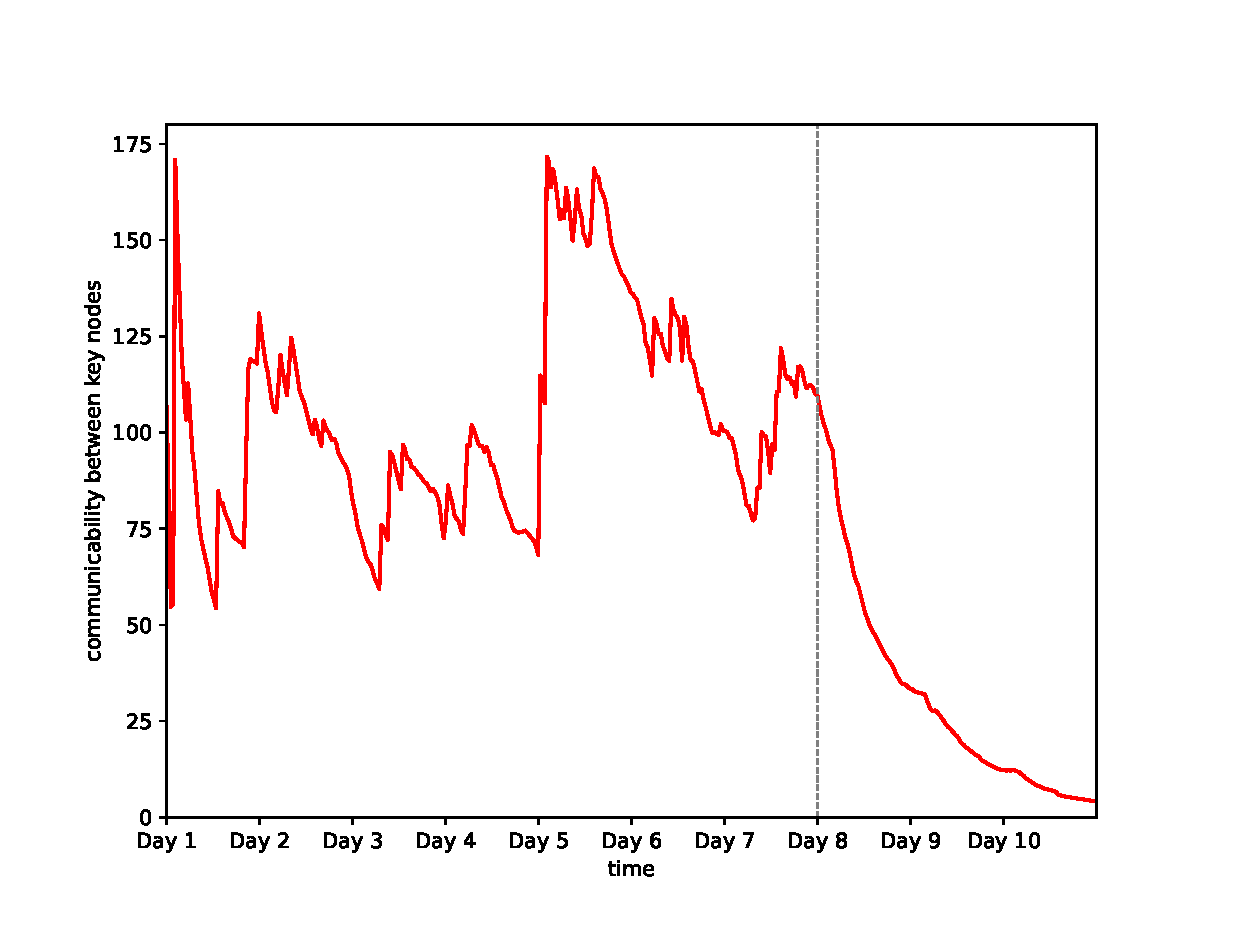
\includegraphics[width=.85\textwidth]{voicecall_exp_dyncomm}
    \caption{Voice call data: dynamic communicability between the five key nodes as a function of time.}
    \label{fig:ve2}
    \bigskip
\end{figure}